%\documentclass[12pt, openany, twoside]{report}      % paper size is in preamble.sty
\documentclass[12pt, openany]{report}      % paper size is in preamble.sty

%\usepackage[utf8x]{inputenc}
%\renewcommand*\sfdefault{ugq}
\usepackage[T1]{fontenc}
\usepackage{lmodern}
\usepackage{graphicx}
\usepackage{booktabs}
\usepackage{amsfonts}
\usepackage{multicol}
\usepackage{hyperref}
\usepackage{microtype}
\usepackage{lettrine}
%\usepackage[a4paper]{geometry}
\usepackage[top=1in, bottom=1.25in, left=0.5in, right=0.5in]{geometry}

\def\TITLE{NORDAN 26}
\def\SUBTITLE{Nordic Complex Analysis Meeting}
\def\LOCATION{Hella, Iceland -- May 23-25, 2025}

\begin{document}
\begin{titlepage}
    \centering
    %\vpspace{3cm}
    
\includegraphics[scale = 0.45]{figs/title} \\
    \vspace{0.5cm}
    {\Huge \textrm{\SUBTITLE}\par}
    \vspace{0.5cm}
    {\Large \textsl{\LOCATION}\par}
    \vspace{2cm}
    \vfill
    \vfill
    \vfill
    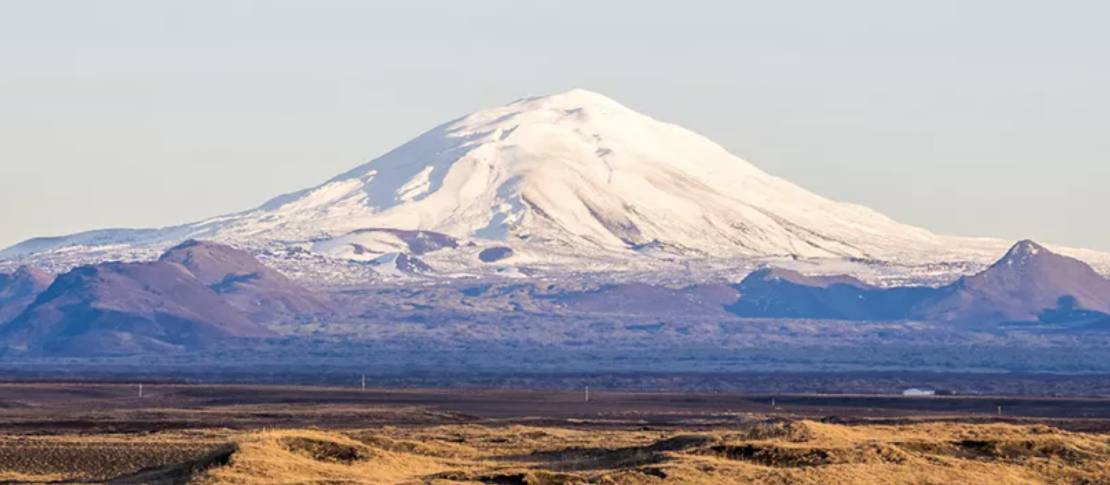
\includegraphics[width=0.8\textwidth]{figs/cover_crop}\par\vspace{1cm}
	\vspace{-1cm}\emph{Hekla, drottning íslenskra eldfjalla}
    \vfill
\end{titlepage}

\newpage
\thispagestyle{empty}

\begin{center}
%    \noindent
%    \fbox{
%        \begin{minipage}{0.7\textwidth}
%            Fjórða Nordan ráðstefnan sem haldin er á Íslandi, og sú 26.
%            í röðinni, er haldin á Hellu með útsýni yfir Heklu, drottningu íslenskra eldfjalla, og Eyjafjallajökul.
%            Ráðstefnan er til heiðurs Jóni Ingólfi Magnússyni og Ragnari Sigurðssyni sem nýlega fóru á eftirlaun.
%            Eftir fyrirlestra laugardagsins er ráðgert að fara inn í Þórsmörk,
%                þar sem hægt er að ganga á Valahnúk og litið verður á fossa í bakaleiðinni.
%        \end{minipage}
%    }

\setlength{\fboxrule}{1.5 pt}
\setlength{\fboxsep}{3 pt}
\vspace{10em}
    \noindent
    \fbox{%
        \setlength{\fboxrule}{0.75 pt}%
        \setlength{\fboxsep}{7 pt}%
        \fbox{%
            \begin{minipage}{0.71\textwidth}
                \lettrine{E}{ftir} áratugsfjarveru verður 26.~Nordan ráðstefnan haldin á Íslandi.
                Þetta er í fjórða skipti sem hún er haldin hér og fá nú gestir að dvelja á Hellu
                    undir vökulum augum Heklu, drottningu íslenskra eldfjalla.
                Ráðstefnan er til heiðurs Jóni Ingólfi Magnússyni og Ragnari Sigurðssyni sem nýlega fóru á eftirlaun.
                Eftir fyrirlestra laugardagsins fer hópurinn með rútu í Þórsmörk,
                    þar sem áhugasömum gefst kostur á að klífa Valahnúk.
                Aðrir geta spókað sig um í sólinni,
                    sjái hún sér fært að mæta,
                    í einni af helstu náttúruperlum Íslands.
                Á leiðinni aftur til Hellu verður viðkoma við Seljalandsfoss.
            \end{minipage}
        }%
    }
\end{center}
    
\vfill


\pagebreak
\renewcommand{\arraystretch}{1.2}
%\usepackage[top=1in, bottom=1.25in, left=0.5in, right=0.5in]{geometry}
\newgeometry{top = 1 in}

\noindent
{\LARGE Program}

\bigskip
\bigskip
\noindent
\textbf{\large Friday, May 23rd}
\smallskip

\noindent
\begin{tabular}{l@{\ } l@{\ } l l}
18:00 & - & 20:00 & \textit{Bus trip to Hella}
\end{tabular}

\bigskip
\noindent
\textbf{\large Saturday}
\smallskip

\noindent
\begin{tabular}{l@{ } l@{ } l l}
09:00 & - & 09:50 & \textsc{Finnur Lárusson}
\\
09:50 & - & 10:20 & \textit{Break}
\\
10:20 & - & 11:10 & \textsc{Daniel Barlet}
\\
11:10 & - & 12:00 & \textsc{Arkadiusz Lewandowski}
\\
12:00 & - & 13:00 & \textit{Lunch}
\\
13:00 & - & 13:50 & \textsc{Mats Andersson}
\\
15:00 &  &  & \textit{Excursion}
\end{tabular}

\bigskip
\noindent
\textbf{\large Sunday}
\smallskip

\noindent
\begin{tabular}{l@{ } l@{ } l l}
09:00 & - & 09:50 & \textsc{Olof Rubin}
\\
09:50 & - & 10:20 & \textit{Break}
\\
10:20 & - & 11:10 & \textsc{Gianmarco Brocchi}
\\
11:10 & - & 12:00 & \textsc{Sibel Şahin}
\\
12:00 & - & 13:00 & \textit{Lunch}
\\
13:00 & - & 13:50 & \textsc{Tyson Ritter}
\\
13:50 & - & 14:40 & \textsc{Jouni Rättyä}
\\
16:00 & - & 18:00 & \textit{Bus trip to Reykjavík}
\end{tabular}

\vfill
\vfill
\noindent
Organizers:
\begin{itemize}
    \setlength\itemsep{-0.3 em}
    \item Benedikt Steinar Magnússon, University of Iceland
    \item Álfheiður Edda Sigurðardóttir, IMFM, Ljubljana
    \item Bergur Snorrason, University of Iceland
    \item Gianmarco Brocchi, University of Iceland
\end{itemize}

\noindent
Conference webpage: \url{https://nordan-conference.github.io/}
\vfill

\cleardoublepage

\newcommand\talk[3]{%
    \vspace{3 ex}
    \noindent
    \textsc{\large #1}

    \smallskip
    \noindent
    \textbf{\textit{#2}}

    \medskip
    \noindent
    #3

}

\talk{Gianmarco Brocchi}{Progress on the Kate square root estimate}
{%
    The Kato square root estimate is a $L^2$ inequality concerning
    perturbations of the Laplacian. While the one-dimensional case was
    established in the 1980s by Coifman, McIntosh, and Meyer,
    the higher-dimensional extension — where the perturbation takes the
    form of a matrix-valued function $A$ in the divergence-form operator
    $-\mathrm{div}(A \nabla)$ — remained open for two more decades.

    In this talk, I will introduce the Kato square root estimate and
    describe the \emph{first-order method}, a technique that reduces the
    second-order operator $-\mathrm{div}(A \nabla)$ to a first-order,
    bisectorial operator $DB$. This method exploits a connection between
    harmonic and holomorphic extensions and allows us to rewrite the
    original estimate as a question about the boundedness of the
    holomorphic functional calculus for $D B$.

    I will also present recent results in the theory, including extensions
    to Riemannian manifolds and to operators with \emph{degenerate
    coefficients}, where the matrix $A(x)$ may lack uniform bounds or
    accretivity and can exhibit singular behaviour. What types of
    singularities can be handled? On which classes of manifolds? And in
    Euclidean space, can one treat anisotropic singularities, namely
    those that vary with direction? 

    New results are part of ongoing joint work with Andreas Rosén.  
}

\talk{Jouni Rättyä}{Carleson measures for Bergman spaces}
{%
    A positive Borel measure $\mu$ on the unit disc is called the
    $q$-Carleson measure for the Bergman space $A^p_\omega$ if
    the identity mapping from $A^p_\omega$ to the Lebesgue space
    $L^q_\mu$ is bounded. In this talk we give an overview of these
    measures in the case when $\omega$ is a radial doubling weight
    in the unit disc and show a number of applications of these
    measures. At the end of the talk we pose a few open problems
    related to the less understood case of non-radial weights.
}


\talk{Tyson Ritter}{A Rudin-Carleson theorem with Runge approximation for maps into Oka manifolds}
{%
    Given a closed set $E \subset \partial {\mathbb D}$ of measure
    zero and a continuous function $\varphi: E \to {\mathbb C}$, the
    classical Rudin-Carleson theorem states that there exists a
    continuous function $F : \overline {\mathbb D} \to {\mathbb C}$
    that is holomorphic on ${\mathbb D}$ and satisfies
    $F|_E = \varphi$. In this talk I will present a
    generalisation of the Rudin-Carleson theorem for maps into Oka
    manifolds that additionally includes approximation on compact
    subsets $K \subset {\mathbb D}$ without any holes and
    interpolation at a point $c \in {\mathbb D}$. This is joint work
    in progress with Benedikt Magnússon (University of Iceland).
}

\pagebreak
\talk{Arkadiusz Lewandowski}{Exposing type results for smoothly bounded (strictly)\\pseudoconvex domains}
{%
    It is well known that every boundary point of a strictly
    pseudoconvex domain admits an exposing mapping. We shall discuss
    the difficulties, possibilities, and tools that appear when
    trying to extend this kind of result beyond the class of
    strictly pseudoconvex smoothly bounded domains.
}

\talk{Daniel Barlet}{Geometric flatness: from the proper case to the non proper case}
{%
    After recalling the case of proper maps, I shall discuss the non
    proper case giving a survey of our recent work with Jon Magnusson
    on the use of finite type cycles in complex geometry.
}


\talk{Sibel Şahin}{Approximation Numbers: From Kolmogorov Numbers\\to Differences of Composition Operators}
{
    Joint work with Frédéric Bayart of Laboratoire de Mathématiques Blaise Pascal.

    In this talk we will first consider various singular numbers of operators
    which happen to be equivalent in the Hilbert space setting. Through
    Kolmogorov numbers we will first see how these singular entities for
    composition operators relate to complex potential theory, namely
    Monge-Amp`ere capacity. In the second part we will relate the component
    structure of bounded composition operators to the function theoretic
    properties of the symbols and for this we will focus on the approximation
    numbers of differences of composition operators. We will see how one can
    obtain optimal upper and lower bounds for approximation numbers of
    differences using classical singular invariants like Bernstein and
    Gelfand numbers and specific choices of Blaschke products from the
    underlying function space.

    \bigskip
    \noindent
    \textit{\textbf{\large Literature}}

    \medskip
    \textsc{G. Lechner, D. Li, H. Queffélec, L. Rodriguez-Piazza}
    
    \hfill \textit{Approximation numbers of weighted composition operators}

    \hfill Journal of Functional Analysis 274, 1928–1958 (2018)

    \textsc{J. Moorhouse, C. Toews}
    \hfill \textit{Differences of composition operators}

    \hfill Contemporary Mathematics 321, 207–213 (2003)

    \textsc{H. Queffélec, K. Seip}
    \hfill \textit{Decay rates for approximation numbers}

    \hfill \textit{of composition operators}

    \hfill Journal d’Analyse Mathématique 125, 371–399 (2015)%
}

\pagebreak
\talk{Mats Andersson}{Singular metrics on holomorphic vector bundles}
{%
    Let $E\to X$ be a holomorphic vector bundle over a complex
    manifold $X$. I will discuss how one can define Chern form,
    Segre form and curvature tensor, associated with a class of
    singular metrics on $E$. I will also present some recent results
    in joint works in progress with Kalm, Lärkäng, and Sera.
}


\talk{Olof Rubin}{Chebyshev polynomials on equipotential curves}
{%
    Given a compact set $K\subset \mathbb C$, a Chebyshev polynomial
    is a monic polynomial that minimizes the supremum norm on $K$.
    When $K$ is infinite such a polynomial exists uniquely for each
    degree. Although there are no explicit formulas for computing
    Chebyshev polynomials, they can be studied through families of
    near-minimal polynomials. One such family is that of Faber
    polynomials, which arise naturally from the conformal map of the
    complement of $K$ onto the exterior of the unit disk. In this
    talk, I will present recent results establishing connections
    between Chebyshev and Faber polynomials on equipotential curves.
}

\talk{Finnur Lárusson}{Holomorphic and algebraic immersed curves directed by a flexible cone}
{%
    I will describe recent joint work with Antonio Alarcón
    (Crelle 2025) and Alarcón and Franc Forstnerrič (arXiv 2024).
    We investigate immersed complex curves in complex affine space,
    directed by a cone $A$ satisfying one of the flexibility
    properties that are studied in Oka theory. When $A$ is the
    so-called null quadric, such curves play a fundamental role in
    the theory of minimal surfaces. There are other important
    examples.  We are interested in approximation and interpolation
    theory for such curves, as well as the ``rough shape'' of the
    space of all curves. I will review results from 5-10 years ago
    in the holomorphic case and then describe our recent results in
    the algebraic setting, where obstacles not present in the
    holomorphic case arise.
}



\newpage
\newgeometry{top = 0.5 in}

\noindent
{\LARGE Participants}

\bigskip
\bigskip
\noindent
\textbf{Alexander Rashkovskii} -
\textit{Universitetet i Stavanger}
\\
\textbf{Ai My Aleksandra Le} -
\textit{Lund University}
\\
\textbf{Álfheiður Edda Sigurðardóttir} -
\textit{IMFM}
\\
\textbf{Andreas Lind} -
\textit{Mittuniversitetet}
\\
\textbf{Antti Perälä} -
\textit{Umeå University}
\\
\textbf{Arkadiusz Lewandowski} -
\textit{Jagiellonian University}
\\
\textbf{Atte Pennanen} -
\textit{University of Eastern Finland}
\\
\textbf{Aurélio Menegon Neto} -
\textit{Mittuniversitetet}
\\
\textbf{Benedikt Steinar Magnússon} -
\textit{Háskóli Íslands}
\\
\textbf{Benjamin Marim de Moura} -
\textit{Mittuniversitetet}
\\
\textbf{Beno Učakar} -
\textit{IMFM}
\\
\textbf{Bergur Snorrason} -
\textit{Háskóli Íslands}
\\
\textbf{Breki Pálsson} -
\textit{Háskóli Íslands}
\\
\textbf{Daniel Barlet} -
\textit{Institut Élie Cartan De Lorraine}
\\
\textbf{Eggert Karl Hafsteinsson} -
\textit{Menntaskólinn í Reykjavík}
\\
\textbf{Erik Avelin} -
\textit{Stockholm University}
\\
\textbf{Fani Xerakia} -
\textit{University of Vienna}
\\
\textbf{Finnur Lárusson} -
\textit{University of Adelaide}
\\
\textbf{Gaofeng Huang} -
\textit{University of Bern}
\\
\textbf{Gianmarco Brocchi} -
\textit{Háskóli Íslands}
\\
\textbf{Håkan Samuelsson Kalm} -
\textit{Chalmers and Gothenburg University}
\\
\textbf{João Fontinha} -
\textit{University of Lisbon}
\\
\textbf{Johannes Testorf} -
\textit{NTNU}
\\
\textbf{Jón Ingólfur Magnússon} -
\textit{Háskóli Íslands}
\\
\textbf{Jouni Paavo Sammeli Rättyä} -
\textit{University of Eastern Finland}
\\
\textbf{Ludvig Svensson} -
\textit{Chalmers and Gothenburg University}
\\
\textbf{Mar Saiz Aparicio} -
\textit{Universitetet i Stavanger}
\\
\textbf{Margaret Stawiska-Friedland} -
\textit{AMS/Mathematical Reviews}
\\
\textbf{Mårten Nilsson} -
\textit{Stockholm University}
\\
\textbf{Mats Andersson} -
\textit{Chalmers and Gothenburg University}
\\
\textbf{Michał Kudra} -
\textit{Jagiellonian University}
\\
\textbf{Olof Rubin} -
\textit{Lund University}
\\
\textbf{Przemysław Sprus} -
\textit{Jagiellonian University}
\\
\textbf{Ragnar Sigurðsson} -
\textit{Háskóli Íslands}
\\
\textbf{Rahim Nkunzimana} -
\textit{Chalmers and Gothenburg University}
\\
\textbf{Risto Korhonen} -
\textit{University of Eastern Finland}
\\
\textbf{Rolf Andreasson} -
\textit{Gothenburg University}
\\
\textbf{Setareh Eskandari} -
\textit{Umeå University}
\\
\textbf{Sibel Şahin} -
\textit{Mimar Sinan Güzel Sanatlar Üniversitesi}
\\
\textbf{Suprokash Hazra} -
\textit{Mittuniversitetet}
\\
\textbf{Tryggvi Kalman Jónsson} -
\textit{Háskóli Íslands}
\\
\textbf{Tyson Ritter} -
\textit{Universitetet i Stavanger}
\\
\textbf{Wills Ton Minh Nguyen} -
\textit{IMFM}
\restoregeometry

\newpage

\begin{center}
    \begin{tabular}{llll}
        \toprule
        \multicolumn{4}{c}{Nordan - Nordic Complex Analysis Meeting}\\
        \midrule
         & Year & Location & Organizers \\
         \midrule
        1 & 1997 & Trosa & Stockholm University  \\
        2 & 1998 & Marstrand & Chalmers University of Technology/\\
          &      &               & University of Gothenburg \\
        3 & 1999 & Saltsjöbaden & Stockholm University  \\
        4 & 2000 & Örnköldsvik & Mid Sweden University/Umeå University\\
        5 & 2001 & Voksenåsen & University of Oslo \\
        6 & 2002 & Reykjavik & University of Iceland \\
        7 & 2003 & Visby & Stockholm University\\
        8 & 2004 & Nösund, Orust & Chalmers University of Technology/\\
           &      &               & University of Gothenburg \\
        9 & 2005 & Sigtuna & Uppsala University \\
        10 & 2006 & Sundsvall & Mid Sweden University/Umeå University \\
        11 & 2007 & Drøbak & University of Oslo\\
        12 & 2008 & Mariehamn, Åland & Stockholm University - Part of the Mittag-Leffler program\\
        13 & 2009 & 
        Reykholt & University of Iceland\\
        14 & 2010 & Lökeberg & Chalmers University of Technology/\\
           &      &               & University of Gothenburg\\
        15 & 2011 & Röstånga & Lund University\\
        16 & 2012 & Kiruna & Mid Sweden University/Umeå University\\
        17 & 2013 & Svolvær & University of Oslo\\
        18 & 2014 & Luminy & CIRM - Nordan+Kawa\\
        19 & 2015 & Reykjavik & University of Iceland\\
        20 & 2016 & Stockholm & Part of the 27th Nordic Congress of Mathematics\\
        21 & 2017 & Tollered & Chalmers University of Technology/\\
           &      &               & University of Gothenburg\\
        22 & 2018 & Hjelmeland & University of Stavanger\\
        23 & 2019 & Lunteren & University of Amsterdam\\
        24 & 2023 & Rydebäck & Lund University\\
        25 & 2024 & Östanskär & Mid Sweden University/Umeå University\\
        26 & 2025 & Hella & University of Iceland\\
    %    27 & 2026 & TBA & University of Eastern Finland & NaN & NaN & NaN & NaN & NaN \\
        \bottomrule
    \end{tabular}
\end{center}
    
\begin{center}
    \begin{tabular}{llll}
        \toprule
        \multicolumn{4}{c}{KAUS - Complex Analysis without Seniors}\\
        \midrule
         & Year & Location & Organizers \\
         \midrule
        1 & 2005 & Umeå & Umeå University\\
        2 & 2006 & Göteborg  & Chalmers University of Technology/\\
          &      &               & University of Gothenburg \\
        3 & 2007 & Sundsvall & Mid Sweden University\\
        4 & 2008 & Stockholm & Stockholm University  \\
        5 & 2009 & Reykjavík & University of Iceland\\
        6 & 2010 & Umeå & Umeå University\\
        7 & 2011 & Göteborg & Chalmers University of Technology/\\
           &      &               & University of Gothenburg\\
        8 & 2024 & Östanskär & Mid Sweden University/Umeå University\\
        9 & 2025 & Reykjavík & University of Iceland\\
    %    27 & 2026 & TBA & University of Eastern Finland & NaN & NaN & NaN & NaN & NaN \\
        \bottomrule
    \end{tabular}
\end{center}
\end{document}


